\section{Design}
In this section we will first discuss an high-level design (\ref{sec:high-level})
and then propose some optimizations (\ref{sec:optimizations}).

\subsection{High-level design idea}
\label{sec:high-level}

\begin{figure}[h!]
  \centering
  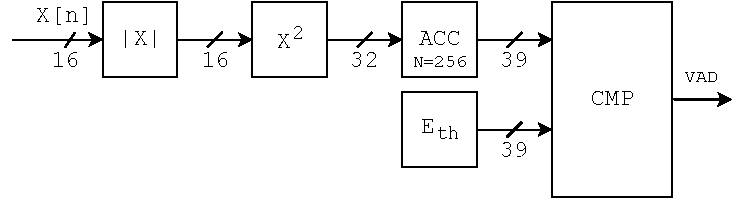
\includegraphics{figs/vad_simple_schematic.pdf}
  \caption{High-level schematic of our VAD design.}
  \label{fig:simple_schematic}
\end{figure}

\cref{fig:simple_schematic} shows the high-level concept of the design, where we 
can see:
\begin{itemize}
  \item \texttt{absnetwork}: a combinatorial network that extracts $|z|$. Both 
    its input and its output have 16 bits since its maximum value is $2^{15}$. 
    In \cref{sec:opt-abs}, we will evaluate whether to use an approximated 
    but more efficient \texttt{absnetwork} that does not sum 1 to the complement.
  \item \texttt{squarepowernetwork}: a combinatorial network that evaluates
    $|z|^2$ on 32 bits. Note that, 31 bits would be enough since 
    $|z|^2 \le (2^{15})^2 = 2^{30}$.
  \item \texttt{accumulator}: performs the recursive sum $S[n] = |z[n]|^2 + S[n - 1]$.
    The maximum sum value is $N \cdot 2^{30} = 256 \cdot 2^{30} = 2^{38}$, 
    requiring 39 bits.
  \item \texttt{comparator}: combinatorial network that compares the output
    of the \texttt{accumulator} with $E_{th}'$, which must be represented on 39
    bits as well in order to be compared to the sum.
\end{itemize}

\subsection{Optimizations}
\label{sec:optimizations}

In order to reduce the number of resources used in the implementation, we can
check for possible optimizations.

\subsubsection{Comparison}
We note that $E_{th}' \simeq 13743895347$ and $\lceil\log_2 E_{th}' + 1\rceil = 34$.
This means that 34 bits would be enough to represent $E_{th}'$. This also implies
that we don't need the accumulator to sum up to more than $2^{34} - 1$, because
if the sum exceeds $2^{34}$, the sum is grater than the threshold.

Moreover we can initialize the initial value of the sum to the overflow value
minus the threshold, so that the overflow will indicate that the threshold has
been exceeded, without using the comparator logic. The initial value of the sum
is $S'[0] = 2^{34} - E'_{th} = 3435973837$ and we compute:
\begin{align*}
  S'[n] &= \bigg| S'[n-1] + |z[n]|^2 \bigg|_{2^{34}}\\
  ovf[n] &= \bigg\lfloor \frac{S'[n-1] + |z[n]|^2}{2^{34}} \bigg\rfloor
\end{align*}
$ovf[n] = 1$ does not imply that $ovf[n + 1] = 1$, but since we are summing
positive integers, the sum will obviously exceed $2^{34}$, so we must remember
that the threshold has been exceeded until the end of the frame.
For this purpose we used a Set-Reset Flip Flop, which is reset at the beginning
of the frame processing and eventually set by $ovf[n]$.

\subsection{Absolute value}
\label{sec:opt-abs}

Calling Z the representation of $z[n]$ on 16 bits, we have that:
\begin{equation}
  |Z| = \begin{cases}
    Z & z[n] \ge 0 \\
    \bar{Z}+1 & z[n] < 0
  \end{cases}
\end{equation}
where $\bar{Z}$ is the complement of $Z$.

In order to simplify it, we could avoid adding 1 in the lower branch, achieving 
two optimizations: a lower number of bits for the output (15 vs 16) and a 
simpler logic.

\begin{equation}
  |Z| \simeq \begin{cases}
    Z & z[n] \ge 0 \\
    \bar{Z} & z[n] < 0
  \end{cases}
\end{equation}

This approximation introduces an error on the energy of the sample. 
This error for negative $x[n]$ can be evaluated as
\begin{equation}
  \epsilon[n] = |z[n]|^2 - \tilde{z}^2[n] = (\bar{Z}[n] + 1)^2 - \bar{Z}^2[n] = 2\bar{Z}[n] + 1
\end{equation}
The worst error we can make on one sample corresponds to $\bar{Z}[n] = 2^{15}$
so $\epsilon_{max} = 2^{16}+1$, which translates to a maximum error on the total 
energy of $256 \cdot \epsilon_{max} \simeq 2^{24}$, which is $\sim 0.12\%$ of the 
threshold. 

In conclusion, the approximation can be safely introduced in order to save 
resources on the FPGA.

\subsection{Clock and sampling}
The sampling rate is 16\si{\kilo\hertz}, but we can process the data at a faster
rate. If we used a 16\si{\kilo\hertz} clock and after a frame is processed,
another one followed, a clock cycle would be required for \texttt{FRAME\_START}.
So we loose a clock cycle at every frame. In order to avoid so, we could use a
faster clock and divide it, so that one short clock cycle is spent in resetting
everithing at the \texttt{FRAME\_START}, but more clock cycles are
available to process the current input sample before it changes.

In order to perform the clock frequency division a properly configured counter 
has been used. The overflow of the counter is used to enable the accumulator, 
which must accumulate at a rate equal to the sampling one.
The accumulation should occur at instants which are in the middle of two sample
instants in order to improve reliability.
